\documentclass{standalone}
\usepackage{../../../../preamble_tikz}

\begin{document}
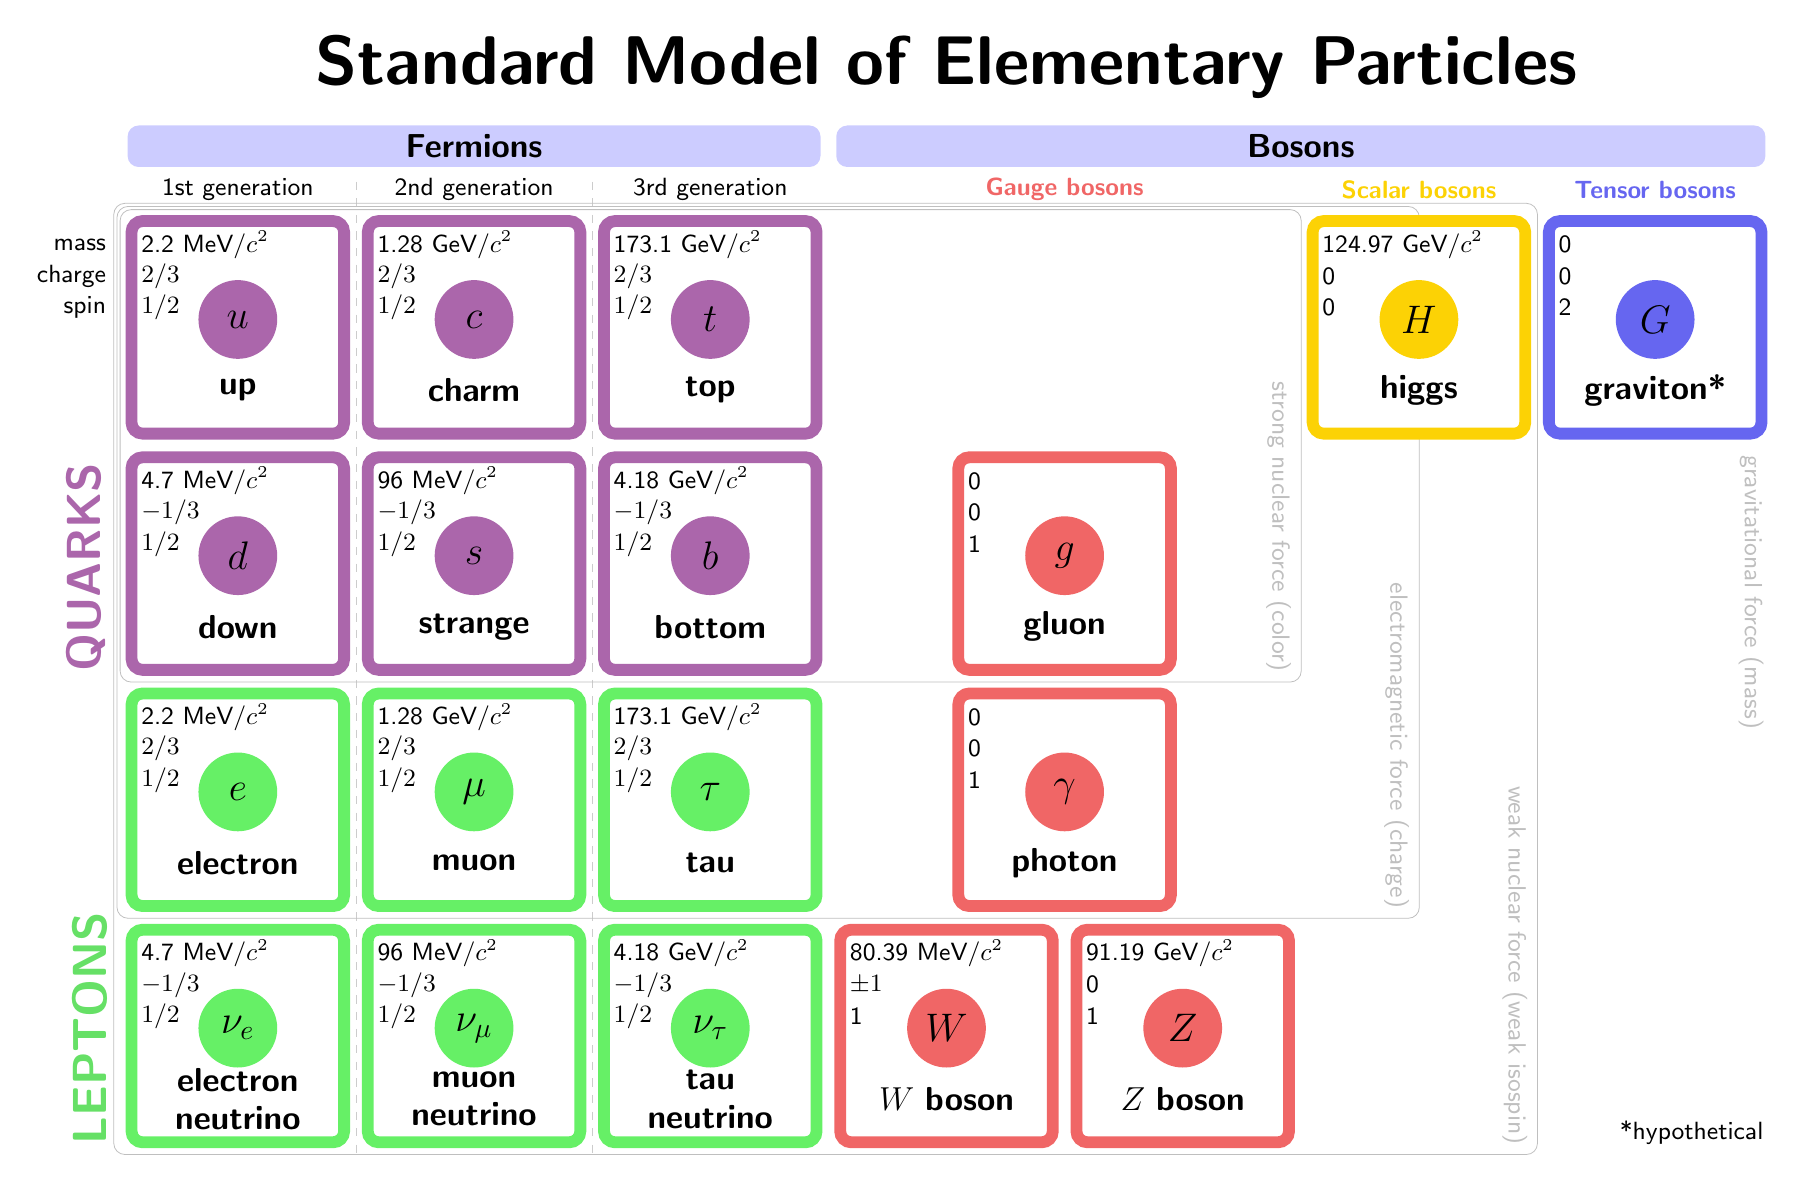
\begin{tikzpicture}
  \sffamily
  \def\particle#1#2#3#4#5#6#7#8{
    \node[rectangle,line width=1.5mm,minimum width = 3cm,minimum height = 3cm] at (#3,#4){};
    \node[rectangle,draw=#1,line width=1.5mm,fill=white,minimum width = 2.7cm,minimum height = 2.7cm,rounded corners] (#2) at (#3,#4){};
    \node[circle,fill=#1,minimum size = 1cm,font=\Large] at (#3,#4+0.1){#5}; %minimum size = diameter of the circle.
    \node[anchor=center,font=\large,text width=2cm, align=center] at (#3,#4-0.8){\textbf{#2}};
    \node[anchor=west,font=\small] at (#3-1.35,#4+1.05){#6};
    \node[anchor=west,font=\small] at (#3-1.35,#4+0.65){#7};
    \node[anchor=west,font=\small] at (#3-1.35,#4+0.25){#8};
    % \node[anchor=north,font=\small] at (#3,#4-0.4){#8};
  }

  \node[anchor=east,font=\small] at (-1.55,1.05){mass};
  \node[anchor=east,font=\small] at (-1.55,0.65){charge};
  \node[anchor=east,font=\small] at (-1.55,0.25){spin};

  \node[rectangle,minimum width = 21cm,minimum height = 1cm,font=\Huge] at (9,3.3){\textbf{Standard Model of Elementary Particles}};
  \node[rectangle,fill=blue!20,minimum width = 8.8cm,minimum height = 0.5cm,font=\large, rounded corners] at (3,2.3){\textbf{Fermions}};
  \node[rectangle,fill=blue!20,minimum width = 11.8cm,minimum height = 0.5cm,font=\large, rounded corners] at (13.5,2.3){\textbf{Bosons}};

  \node[font=\small] at (0,1.75){1st generation};
  \draw[very thin, dashed, gray!40] (1.5,1.85) -- (1.5,-10.5);
  \node[font=\small] at (3,1.75){2nd generation};
  \draw[very thin, dashed, gray!40] (4.5,1.85) -- (4.5,-10.5);
  \node[font=\small] at (6,1.75){3rd generation};

  \node[font=\small, red!90!black!60] at (10.5,1.75){\textbf{Gauge bosons}};
  \node[font=\small, yellow!70!orange] at (15,1.75){\textbf{Scalar bosons}};
  \node[font=\small, blue!90!black!60] at (18,1.75){\textbf{Tensor bosons}};


  %interactions
  \node[rectangle,anchor=north west,draw=gray!50,line width=0.1mm,minimum width = 15cm,minimum height = 6cm,rounded corners] (rgluon) at (-1.5,1.5){};
  \node[anchor=north east,font=\small,rotate=270,gray!50!] at (13.5,-4.5){strong nuclear force (color)};
  \node[rectangle,anchor=north west,draw=gray!50,line width=0.1mm,minimum width = 16.54cm,minimum height = 9.04cm,rounded corners] at (-1.54,1.54){};
  \node[anchor=north east,font=\small,rotate=270,gray!50!] at (15,-7.5){electromagnetic force (charge)};
  \node[rectangle,anchor=north west,draw=gray!50,line width=0.1mm,minimum width = 18.08cm,minimum height = 12.08cm,rounded corners] at (-1.58,1.58){};
  \node[anchor=north east,font=\small,rotate=270,gray!50!] at (16.5,-10.5){weak nuclear force (weak isospin)};
  \node[anchor=north west,font=\small,rotate=270,gray!50!] at (19.5,-1.5){gravitational force (mass)};

  %QUARKS
  \node[anchor=south west,font=\LARGE,rotate=90,violet!90!black!60] at (-1.55,-4.5){\textbf{QUARKS}};

  \particle{violet!90!black!60}{up}{0}{0}{$u$}{2.2 MeV/$c^2$}{$2/3$}{$1/2$}
  \particle{violet!90!black!60}{down}{0}{-3}{$d$}{4.7 MeV/$c^2$}{$-1/3$}{$1/2$}
  \particle{violet!90!black!60}{charm}{3}{0}{$c$}{1.28 GeV/$c^2$}{$2/3$}{$1/2$}
  \particle{violet!90!black!60}{strange}{3}{-3}{$s$}{96 MeV/$c^2$}{$-1/3$}{$1/2$}
  \particle{violet!90!black!60}{top}{6}{0}{$t$}{173.1 GeV/$c^2$}{$2/3$}{$1/2$}
  \particle{violet!90!black!60}{bottom}{6}{-3}{$b$}{4.18 GeV/$c^2$}{$-1/3$}{$1/2$}

  %LEPTONS
  \node[anchor=south west,font=\LARGE,rotate=90,green!80!black!60] at (-1.55,-10.5){\textbf{LEPTONS}};

  \particle{green!90!black!60}{electron}{0}{-6}{$e$}{2.2 MeV/$c^2$}{$2/3$}{$1/2$}
  \particle{green!90!black!60}{electron neutrino}{0}{-9}{$\nu_e$}{4.7 MeV/$c^2$}{$-1/3$}{$1/2$}
  \particle{green!90!black!60}{muon}{3}{-6}{$\mu$}{1.28 GeV/$c^2$}{$2/3$}{$1/2$}
  \particle{green!90!black!60}{muon neutrino}{3}{-9}{$\nu_\mu$}{96 MeV/$c^2$}{$-1/3$}{$1/2$}
  \particle{green!90!black!60}{tau}{6}{-6}{$\tau$}{173.1 GeV/$c^2$}{$2/3$}{$1/2$}
  \particle{green!90!black!60}{tau neutrino}{6}{-9}{$\nu_\tau$}{4.18 GeV/$c^2$}{$-1/3$}{$1/2$}

  %BOSONS
  \particle{red!90!black!60}{gluon}{10.5}{-3}{$g$}{0}{0}{1}
  \particle{red!90!black!60}{photon}{10.5}{-6}{$\gamma$}{0}{0}{1}
  \particle{red!90!black!60}{$Z$ boson}{12}{-9}{$Z$}{91.19 GeV/$c^2$}{0}{1}
  \particle{red!90!black!60}{$W$ boson}{9}{-9}{$W$}{80.39 MeV/$c^2$}{$\pm 1$}{1}

  \particle{yellow!70!orange}{higgs}{15}{0}{$H$}{124.97 GeV/$c^2$}{0}{0}

  \particle{blue!90!black!60}{graviton*}{18}{0}{$G$}{0}{0}{2}
  \node[anchor=south east,font=\small] at (19.5,-10.5){*hypothetical};


\end{tikzpicture}
\end{document}
